\documentclass[11pt]{article}

\usepackage{amsmath}
\usepackage{textcomp}
\usepackage[top=0.8in, bottom=0.8in, left=0.8in, right=0.8in]{geometry}
% Add other packages here %

\usepackage{amssymb}
\usepackage{mathtools}
\usepackage{graphicx}
\usepackage{subcaption}
\usepackage[export]{adjustbox}


% Put your group number and names in the author field %
\title{\bf Excercise 4\\ Implementing a centralized agent}
\author{Group \textnumero$75$: Thomas KIMBLE, Jules AFRESNE}


% N.B.: The report should not be longer than 3 pages %


\begin{document}
\maketitle

\section{Solution Representation}

\subsection{Variables}
% Describe the variables used in your solution representation %

Our solution representation has the following variables:
\begin{itemize}
    \item \textit{vehicles}: A list of all of the simulation vehicles.
    \item \textit{tasks}: A TaskSet of all of the simulation tasks.
    \item \textit{worldNbTasks}: An integer equal to the number of tasks in the simulation.
    \item \textit{worldPlan}: A list of a list to represent each vehicle plan. The sub-list is the pickup or delivery tasks for each vehicle while the main list is of the vehicles themselves. If a pickup task is added, the corresponding delivery task is added $worldNbTasks$ indices after. We get the following for $k$ vehicles and $N_T = worldNbTasks$ tasks:\\ 
    \[ 
    \Big[ \; \big[ task(1)_{v1},  task(2)_{v1},  ..., task(l)_{v1}, ... , task(1+N_T)_{v1},  task(2+N_T)_{v1},  ..., task(l+N_T)_{v1} \big] \Big. ,
    \]
    \[ 
    \\ \; \; \; \;\; \; \; \; \big[ task(1)_{v2},  task(2)_{v2},  ..., task(m)_{v2}, ... , task(1+N_T)_{v2},  task(2+N_T)_{v2},  ..., task(m+N_T)_{v2} \big] ,
    \]
    \[ 
    \\ \\ ... \; ,
    \]
    \[ 
    \\ \; \; \; \; \; \; \; \; \; \Big. \big[ task(1)_{vk},  task(2)_{vk},  ..., task(n)_{vk}, ... , task(1+N_T)_{vk},  task(2+N_T)_{vk},  ..., task(n+N_T)_{vk}  \big] \; \Big]
    \]
\end{itemize}

\subsection{Constraints}
% Describe the constraints in your solution representation %
We have the following constraints:
\begin{itemize}
    \item Two corresponding pickup and delivery tasks must be in the same vehicle.
    \item A delivery task had to be after it's corresponding pickup task.
    \item The added weight of pickup tasks before their delivery in a sub-list must be inferior to the vehicles capacity.
\end{itemize}

\subsection{Objective function}
% Describe the function that you optimise %
First of all we want to minimise the total cost function. For each vehicle we have a distance and a cost per km value. The total cost function is therefore:
$distanceCost = \sum_{vehicles}^{} distance \cdot costPerKm$ \\

\noindent \noindent For our solution also want to minimise the time taken to pickup and deliver all of the tasks. we therefore calculate the time taken for each vehicle to follow its plan and we take the longest time. The time function is therefore: $timeCost = max_{vehicles}(time)$ \\

\pagebreak
\noindent \noindent We therefore combine the two to get the following objective function that we want to minimise. We divide $distanceCost$ by the mean of the vehicle speeds ($meanSpeed$) multiplied by the amount of vehicles ($N_V$) squared to avoid outweighing the $timeCost$. We get the following objective function:
$$Cost = timeCost + distanceCost/(meanSpeed \cdot N_V^2)$$

\section{Stochastic optimisation}

\subsection{Initial solution}
% Describe how you generate the initial solution %
We have three possible initial solutions. The first is to assign the tasks randomly to the vehicles while checking constraints to assure a possible solution (case "$randomly$"). The second is to distribute the tasks evenly to the vehicles, here each vehicle will have the same amount of vehicles more or less one (case "$fairlyDistributed$"). The final is to give all of the tasks in to the vehicle with the largest capacity (case "$toTheBiggest$"). We use a switch case to choose, but our program is initialised with the second initial solution (case "$fairlyDistributed$") because it converges faster to an optimal solution.

\subsection{Generating neighbours}
% Describe how you generate neighbours %
We generate neighbours two different ways. First of all by moving the first task of a vehicle and its corresponding delivery task to a new vehicle. The second method consists in changing the order of the tasks within a vehicle.

\subsection{Stochastic optimisation algorithm}
% Describe your stochastic optimisation algorithm %
After selecting an initial solution (step 1) we then repeat a new step (step 2) until a termination condition is met. Step 2  has the following sub-steps, where after each one we keep the best solution and use it for the next:

\noindent \noindent \textbf{\textit{Sub-Step 1:}} Choose neighbours, This function provides a set of candidate assignment that are close to the current one and could possibly improve it.

\noindent \noindent \textbf{\textit{Sub-Step 2:}} Local Choice, where we with probability $p$ we randomly choose one of the best neighbour solutions, and with probability $1-p$ we return the previous solution. If p is close to 1, the algorithm converges faster but it is easily trapped into a local minimum.

\noindent \noindent \textbf{\textit{Sub-Step 3:}} We save this sub solution if it's the best one so far. If there is no improvement of cost after a certain time, we start over with our initial solution and keep the best sub solution by repeating these sub-steps to find a new best sub solution (skip to step 4 without activating termination condition). If there is no improvement after $x$ best sub solutions, we keep the last one and activate the termination condition. We also have a second termination condition if we are approaching a time out.

\noindent \noindent \textbf{\textit{Sub-Step 4:}} Repeat until termination condition met. Our last solution is the best one.


\section{Results}

\subsection{Experiment 1: Model parameters}
% if your model has parameters, perform an experiment and analyse the results for different parameter values %

\subsubsection{Setting}
% Describe the settings of your experiment: topology, task configuration, number of tasks, number of vehicles, etc. %
% and the parameters you are analysing %
We observe four vehicles in the \textbf{England topology} with thirty tasks to deliver. Each vehicle has the same speed and capacity. We will analyse the parameters concerning the probability and the initialisation mode at the same time by taking the cost as a criterion.

\subsubsection{Observations}
% Describe the experimental results and the conclusions you inferred from these results %
\begin{figure}[ht]
    \centering
    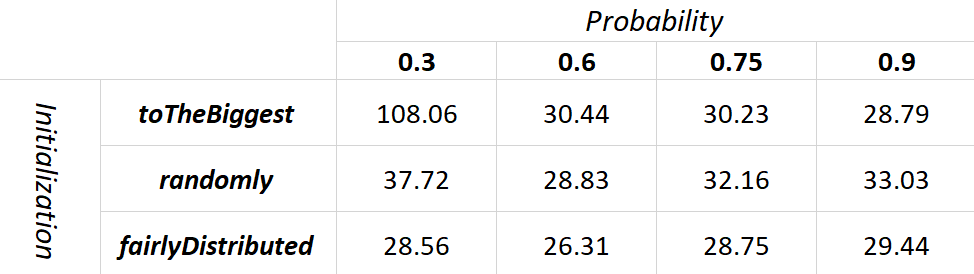
\includegraphics[width=0.55\textwidth, frame]{exp1.PNG}
    \caption{Cost as a function of the initialisation method and probability.}
    \label{fig:1}
\end{figure}

The '$fairlyDistributed$' initialisation with a probability of 0.6 is the most conclusive. Nevertheless, we observe that random initialisation is also interesting but that these performances fluctuate due to the random nature of its initial state. The '$toTheBiggest$' initialisation is not very efficient, moreover we noticed that the computation time is very long with this one.

\subsection{Experiment 2: Different configurations}
% Run simulations for different configurations of the environment (i.e. different tasks and number of vehicles) %

\subsubsection{Setting}
% Describe the settings of your experiment: topology, task configuration, number of tasks, number of vehicles, etc. %
We will use the "$fairlyDistributed$" initialisation in order to have the same initial state for all the experiments. And we set the probability of exploration at 0,6.
We will realise the next four experiments in England topology with vehicles having the same speed and capacity:
\begin{itemize}
    \item 1st: two vehicles and six tasks
    \item 2nd: two vehicles and forty tasks
    \item 3rd: four vehicles and six tasks
    \item 4th: four vehicles and forty tasks
\end{itemize}

\subsubsection{Observations}
% Describe the experimental results and the conclusions you inferred from these results %
% Reflect on the fairness of the optimal plans. Observe that optimality requires some vehicles to do more work than others. %
% How does the complexity of your algorithm depend on the number of vehicles and various sizes of the task set? %
Here are our results for these experiments:
\begin{itemize}
    \item 1st: Cost is equal to $27.68$ and we also notice that only one vehicle has moved.
    \item 2nd: Cost is equal to $98.35$ and both vehicles has moved but not the same duration because it has less tasks than the other.
    \item 3rd: Cost is equal to $10.34$ and we noticed that one vehicle has not moved. In addition, the tasks were unfairly distributed among the vehicles.
    \item 4th: Cost is equal to $38.25$ and all vehicles have moved.
\end{itemize}

We notice a factor of about 4 on the cost when we increase from 6 to 40 tasks with the same number of vehicles. This factor is logical because the distance of the vehicles and therefore the travel time has been increased, but it is not proportional to the increase in the number of tasks because the packages have been grouped together in the cities. We can therefore see that vehicles optimise their routes. Moreover through the experiments we noticed that the more the number of tasks and/or vehicles was increased, the longer the calculation time was. This can be explained by the fact that the algorithm is more complex because it has more choices of state. Finally, we noticed that some vehicles do more actions than others, especially in experiment 2. This can be explained by the fact that the tasks are scattered and that the algorithm considers it unnecessary to engage several vehicles when a single vehicle with an optimised route could have an almost equivalent cost. It is necessary to see if we want to privilege the distance cost or to privilege the speed of delivery or both.

\end{document}